\chapter{Vector space model of optical systems}
\label{ch:modalmodel}
This chapter describes a formalism that treats the laser field components propagating in an optical interferometer as a complex vector space where common optical components, such as mirrors and optical modulators are treated as operators in this space. %NL%
This treatment allows the analysis of complicated optical paths, which include paths that loop onto themselves (as in the case of resonant cavities) to be reduced to a problem of matrix manipulation. %NL%
This is is highly powerful technique which is used extensively in modeling the behavior of gravitational-wave interferometers \cite{Vinet1986,Hefetz:97,Sigg:00}, and is useful for some of the concepts discussed in later chapters.

At this point in the discussion, a bird's eye view of the technique is useful. %NL%
In essence what this formalism provides is a significant abstraction and abbreviation of the effects of opical components (mirrors, modulators, etc.) on the the field components that make up a laser beam. %NL%
In the case of the transverse electric-magnetic (TEM) spatial modes of a laser field, a calculation of how a mirror, which is rotated about some axis perpendicular to the beam, redistributes energy from one field component to another may involve complicated overlap integrals involving the Hermite-Gaussian profiles of the beam modes. %NL%
Such a calculation is difficult to calculate and represent on paper in a concise and transparent way. %NL%
The strength of this technique is that all of these complicated integrals are \emph{baked in} to the linear operators which represent optical components, so to speak. %NL%
All of the involved integral math is performed in the construction of the operators, and is hidden from view when the optical system as a whole is considered. %NL%
What is left is just a problem of linear algebra.

\section{Frequency components of a laser field}
\label{sec:freqspace}
To get a flavor of the formalism, consider the simple example where we choose our vector space to just have three components which represent the amplitude of a carrier frequency field at frequency $\omega_0$, as well as two sideband fields separated in frequency by $\pm\Omega$. %NL%
Consider an electromagnetic wave propagating in the z direction, at some point along the propagation axis, the electric field may be written as
\begin{align*}
\geom{E}(t) &= A_0 e^{i\omega_0t}\geom{x} + A_1e^{i(\omega_0+\Omega)t}\geom{x} + A_{-1}e^{i(\omega_0-\Omega)t}\geom{x}\\
&= \left( A_0 + A_1 e^{i\Omega t}+A_{-1}e^{-i\Omega t}\right) e^{i\omega_0 t}\geom{x},
\end{align*}
where $A_0$, $A_1$ and $A_{-1}$ are the carrier, first order upper sideband and first order lower sideband amplitudes respectively, $k=\omega_0/c$ is the wave-number, and $\geom{x}$ is the \emph{geometrical} basis vector pointing along the axis of polarization. %NL%
We are interested in the vector representation where this same propagating field is represented as\footnote{The use of $\doteq$ in (\ref{eq:dotequals}) is meant to convey that the expression on the right side is a representation of the vector on the left side in the chosen vector space. %NL%
The right side of the equation is not written in terms of vectors and thus is not truly equal to the left side.} 
\begin{equation}
\label{eq:dotequals}
\vect{E} \doteq \ms A_0 \\ A_1 \\ A_{-1} \me.
\end{equation}

The basis vectors in this representation are given by the three periodically time varying components of the electric field, namely the carrier, upper and lower sidebands. %NL%
It is important to emphasize that the vectors used in this formalism are in general not simple euclidean vectors, but rather abstract vectors representing different components of the electric field of an electromagnetic wave. %NL%
The inner product of two basis vectors is:
\[
\inprod{r}{s} = \int\limits_{\text{many cycles}}\! \! \! \! \! \! \! \! \!
\dd t \; \: {\left( e^{i\omega_{r}t}\right)^*}e^{i\omega_{s}t} = \delta_{rs},
\]
where $\omega_r$ is the sideband frequency of the $r$th sideband. %NL%
This treatment is analogous to the formalism of quantum mechanics in which the quantum state of a system is defined by a vector in a space spanned by a set of orthonormal basis state vectors. %NL%
In our formalism, the components of the laser field will take the place of the state vectors. %NL%
We will use Dirac bra-ket notation because of this strong analogy.\footnote{One significant difference between quantum mechanics and this formalism is that the quantum state vector of a system must always have unit length, to ensure the state has a probability of 1. %NL%
The length of the vector in this formalism is just a field amplitude, and can take any value.}

Now that we are familiar with using this vector space to represent the desired wave amplitudes, let's examine how we may use an operator to represent some optical component. %NL%
An electro-optic modulator (EOM) can act as a phase modulator for a laser field when a voltage is applied. %NL%
When a periodic signal is applied at frequency $\Omega$, given an input field amplitude $Ae^{i\omega_0 t}$ (ignoring the $z$ dependence) the output amplitude is
\newcommand{\gammahalf}{\frac{i\Gamma}{2}}
\begin{equation}
\label{eq:inputfield}
Ae^{i\omega_0 t + i\Gamma \cos{\Omega t}}\approx Ae^{i\omega_0 t}\left(1+\gammahalf e^{i\Omega t}+\gammahalf e^{-i\Omega t}\right),
\end{equation}
where $\Gamma$ is known as the modulation depth and is assumed to be small. %NL%
One can show that in the example vector space we are considering, this EOM can be represented as the following operator
\begin{equation}
\oper{\Phi}(\Gamma) \doteq 
\ms 
1          & \gammahalf & \gammahalf \\
\gammahalf & 1          & 0          \\
\gammahalf & 0          & 1 \\
\me.
\end{equation}
It is then clear that the act of $\oper{\Phi}(\Gamma)$ operating on an input field constructed as the one used in (\ref{eq:inputfield}) gives the desired output field:
\begin{equation}
\vect{E_{output}}=
\oper{\Phi}(\Gamma)\vect{E_{\text{input}}} \doteq \ms 
1          & \gammahalf & \gammahalf \\
\gammahalf & 1          & 0          \\
\gammahalf & 0          & 1 \\
\me
\ms A \\ 0 \\ 0 \me = A \ms  1 \\ \gammahalf \\ \gammahalf \me.
\end{equation}

So far, we have kept our example relatively simple. %NL%
The vector space we have chosen represents only the first order sidebands generated on the carrier frequency. %NL%
Also, we have only expanded the effect of phase modulation to terms linear in $\Gamma$. %NL%
There is, however, no fundamental reason that the analysis cannot be extended to arbitrary precision. %NL%
The number of components of the vector space can be expanded to account for an arbitrary number of higher order sidebands, and the matrix elements used for $\oper{\Phi}(\Gamma)$ can take their exact values. %NL%
The general form of the phase modulation operator is:
\begin{equation}
\oper{\Phi}(\Gamma) = \sum_{r,s=-\infty}^\infty\vect{r} i^{s-r} J_{s-r}(\Gamma) \form{s},
\end{equation}
where $\vect{r}$ is the basis vector representing the $r$th order sideband component (which includes a $e^{ir\Omega t}$ time dependence), and $J_k(x)$ is the Bessel function of the first kind.\footnote{This can be shown using the so-called Jacobi-Anger identity, $e^{ix\cos\theta}=\sum_{k=-\infty}^\infty i^kJ_k(x)e^{ik\theta}$. %NL%
Also, $J_{-k}(x)=(-1)^kJ_k(x)$, thus $\oper{\Phi}(\Gamma)$ is symmetric.} The ability to calculate to arbitrary precision will continue to hold true when we expand the treatment to include other components of a propagating laser field, such as the transverse spatial modes. %NL%
As long as the solutions are converging, the precision is only limited by the choice of when the vector space is truncated, i.e.\ to what order the calculation is taken.

\section{The modal space}
\label{sec:modalspace}
So far our example prescribes an elegant way to deal with optical components (e.g.\ the modulator) which transfer energy from one component of the electric field (the carrier) to other components (the sidebands). %NL%
This type of approach is also applicable to the components of the electric field corresponding the the transverse spatial modes of the beam, as shown by \citet{Hefetz:97}.

When the paraxial approximation applies it is possible to expand the electromagnetic field into a superposition of modes represented by a Gaussian function of the transverse coordinate, multiplied by polynomials. %NL%
Common choices for the polynomial functions are the Hermite or Laguerre polynomials \cite[Chap. %NL%
16]{Siegman}. %NL%
This formalism associates the modal components with eigenmodes of what is described as the ``perfectly aligned and undistorted optical path''. %NL%
In other words, this formalism describes how the introduction of misalignments and beam distortions alter a laser beam propagating in the system by treating misalignments (or higher order beam distortions) as matrix elements which transfer energy between different spatial modes. %NL%
The misalignments are generally treated as small, and thus, the operators of the optical components differ from the identity operator by small corrections. %NL%
The misaligned solutions of beam propagation are thus treated as perturbations of the aligned solutions. %NL%


The treatment of modes in this formalism is slightly novel due to the fact that, normally, some fundamental Gaussian laser mode is defined to have a particular beam waist $w_0$, and a focused beam with a different beam waist can be written as a series of higher order components with the original beam waist $w_0$. %NL%
In this formalism, the fundamental Gaussian mode may have a beam waist value that changes due to the presence of a lens, but the beam on both sides of the lens would be represented by the same modal state vector (modulo some phase rotation due to propagation). %NL%
It is only the presence of misalignments and distortions that cause significant off-diagonal matrix elements.

Choosing the common Hermite-Gaussian basis, we can use basis vectors which are separable into the mode order of the beam along the $x$ and $y$ transverse axes of the beam. %NL%
A general field vector can be decomposed in the modal space as
\begin{equation}
\vect{E} = \sum_{m,n=0}^\infty A_{mn}\vect{mn}\doteq\sum_{m,n=0}^\infty A_{mn}U_m(x,z)U_n(y,z)e^{-ikz},
\end{equation}
where $U_m(x,z)$ is the $m$th 1-D Hermite-Gaussian mode (for example, as defined in \citet{Siegman}.) The basis modes are also referred to as the Transverse Electric and Magnetic modes of order $mn$ (\TEM{mn}). %NL%
The Hermite-Gaussian modes form a complete orthonormal set of basis functions, therefore the inner product is $\inprod{mn}{kl}=\delta_{mk}\delta_{nl}$.

In the modal space, a simple example operator would be a mirror that has been tilted by an angle $\theta_x$ about the y axis. %NL%
Due to the mirror misalignment, the phase of the beam at the plane of the mirror has been advanced on one side and retarded on the other side, relative to the aligned beam. %NL%
This can be represented as a phase multiplication of $\exp[-2ik\theta_x x]$. %NL%
\citet{Hefetz:97} show that in the modal basis this is satisfied by the operator
\begin{equation}
\oper{M}(\Theta_x) = \exp\left[ -i\Theta_x\sum_{m,n,k,l=0}^\infty \vect{mn} \delta_{nl} \left( \sqrt k \delta_{m[k-1]}+\sqrt m \delta_{m[k+1]} \right) \form{kl}\right],
\end{equation}
where $\delta_{mn}$ is the Kroneker delta; and $\Theta_x = \theta_x \pi w(z)/\lambda$ is the normalized misalignment angle for beam width $w(z)$ and wavelength $\lambda$, at the beam waist, this is the ratio of the misalignment angle to the beam divergence angle. %NL%
One can see that the $k$ index is connected to the $m$ index that differs by one mode number, this will provide the correct transfer of energy from the \TEM{00} mode to the \TEM{10} mode as discussed above. %NL%
We can use a matrix representation with three components representing the \TEM{00}, \TEM{10} and \TEM{01} amplitudes, explicitly for field $\vect{E}$:
\begin{equation}
\vect{E} \doteq \ms \inprod{00}{E} \\ \inprod{10}{E} \\ \inprod{01}{E} \me
\end{equation}

In this representation, 
\begin{equation}
\label{eqn:mirrortilt}
\oper{M}(\Theta_x) \doteq \exp \left( -i 
\ms 
0 & \Theta_x & 0 \\
\Theta_x & 0 & 0 \\
0 & 0 & 0 
\me
\right)
\approx
\ms
1-\frac{1}{2}\Theta_x^2 & -i\Theta_x& 0 \\
-i\Theta_x & 1-\frac{1}{2}\Theta_x^2& 0 \\
0 & 0 & 1 \\
\me .
\end{equation}
The last approximation being valid for small $\Theta_x$,\footnote{Note that $\theta_x$ being small is also required by the paraxial approximation.}
So for small misalignments, the effect of rotating a mirror is to take energy from the \TEM{00} component of the field, and transfer it to the \TEM{10} component, the opposite also being true when the initial field already has a non-zero \TEM{10} component. %NL%
It is also useful to note that the resulting \TEM{10} field has a quadrature which is rotated by $\pi/2$ with respect to the initial \TEM{00} field. %NL%
Or in other words, the amplitude of the \TEM{10} field is in the \emph{phase direction} relative to the \TEM{00} amplitude.

\section{The combined vector space}
To treat the general problem of laser fields propagating through an optical system, it will be useful to consider both frequency and modal components simultaneously. %NL%
This combination was covered in detail by \citet{Sigg:00}.

Mathematically, the combined space is a tensor product of the spaces discussed above. %NL%
The resulting basis vectors will be labeled by four indices, two from the modal space, one from the frequency space, and for completeness, a final index to represent the polarization. %NL%
We can use the following notation for the basis vectors:
\begin{equation}
\vect{mn;r;p}=\vect{mn}_{\text{modal}}\otimes\vect{r}_{\text{frequency}}\otimes\vect{p}_{\text{polarization}}.
\end{equation}
It is understood that the electric field represented by one of these basis vectors is
\[
\vect{mn;r;p} \doteq e^{\left[ i\left( \omega_0+\omega_r\right)t\right]} U_{mn}\geom{\epsilon}_p,
\]
where $\omega_r$ is some mapping from the index $r$ to a set of frequencies; $U_{mn}$ is shorthand for $U_m(x,z)\times U_n(y,z)$; and $\geom{\epsilon}_p$ for $p\in \{1,2\}$ are the polarization unit vectors in the $x$ and $y$ direction, respectively. %NL%
Note that this treatment handles sidebands slightly different from how they are handled elsewhere. %NL%
For example, \citet{Sigg:00} treat radio frequency modulation sidebands differently from audio frequency sidebands, and also only treat audio frequency sidebands which are regularly spaced. %NL%
Using the treatment outlined here in which all sidebands are treated in the same way and may have arbitrary spacing, we are able to more simply investigate cross modulation products of several modulation sidebands, as well as situations where signal detection frequencies are comparable to modulation frequencies. %NL%
This is accompanied by the sacrifice of potentially having many more matrix elements.

An example of an operator in the combined space is the free space propagation operator:
\begin{align}
\label{eq:Propagator}
\oper{P}(\Delta z,\eta) = & \\
\sum_{\substack{mnkl\\rs\\pq}}& \vect{mn;r;p}
\delta_{mk}\delta_{nl}\delta_{rs}\delta_{pq}
\exp  \left[i(m+n+1)\eta
-i\frac{\omega_0+\omega_r}{c}\Delta z\right] 
\form{kl;s;q}, \notag
\end{align}
using parameters
\begin{align*}
\Delta z &= z_{\text{end}}-z_{\text{start}} \\
\eta &= \arctan \left( \frac{(z_{\text{end}}-z_0)\lambda}{\pi w_0^2}\right)- 
        \arctan \left( \frac{(z_{\text{start}}-z_0)\lambda}{\pi w_0^2}\right)
\end{align*}
for starting and ending positions $z_{\text{start}}$ and $z_{\text{end}}$, where $z_0$ is the position of the beam waist, and $w_0$ is the beam radius at the waist. %NL%
The parameter $\eta$ is commonly referred to as the Gouy phase shift. %NL%
As one can see by the presence of the Kronecker deltas in (\ref{eq:Propagator}), all the components of the input field are directly propagated to the output field without mixing. %NL%
There is, however a phase shift which depends on the transverse mode order (the Gouy shift) and the wavelength ($\omega_r/c$).

More complicated operators exist which simultaneously mix mode and frequency components. %NL%
One example is that of a mirror which is dithered at a given frequency in angle. %NL%
It is in a sense a combination of the misaligned mirror operator in section \ref{sec:modalspace} and the phase modulation operator in section \ref{sec:freqspace}. %NL%
This operator is derived by \citet{Sigg:00}.
\section{Photodetection}
A photodetector is a device which is sensitive to the power in the laser field. %NL%
This is typically photodiode which converts the laser power into an electric current. %NL%
In terms of the electric field we may write the time averaged power incident on a photodiode as
\begin{equation}
\bar{P}=\frac{\epsilon_0 c}{2}\int \! \! \dd t \int \! \! \dd A|E^2|=\frac{\epsilon_0 c}{2}\inprod{E}{E}.
\end{equation}
This fits nicely into our formalism because one can view the average power detected at a photodiode as the squared-norm of the state vector of the laser field. %NL%
Often, however, one may use a photodetector to measure certain frequency components of the power, as well as information about the spatial distribution of the beam. %NL%
Here we outline how to treat such signals in this formalism.

The time dependent components of the laser power can be thought of as the mixing of different frequency components of the electric field. %NL%
To achieve this in the vector space formalism, we must use an operator which has matrix elements connecting different frequency components. %NL%
For demodulation at frequency $\omega_d$, the  operator takes the form: 
\begin{equation}
\label{eqn:fdemodoperator}
\oper{D}(\omega_d) = \sum_{rs} \vect{r} \delta(\omega_r,\omega_s-\omega_d) + \delta(\omega_r,\omega_s+\omega_d)\form{s},
\end{equation}
where we use a delta function defined as
\begin{equation}
\delta(\alpha,\beta) = 
\begin{cases}
0 & \text{if $\alpha \neq \beta$}, \\
1 & \text{if $\alpha = \beta$}.
\end{cases}
\end{equation}
Note that there is a special case where $\omega_d=0$ where $\oper{D}(\omega_d)$ is the identity operator, which does not follow from Equation \ref{eqn:fdemodoperator} and must be handled seperately.
\begin{figure}
  \begin{center}
  \leavevmode
  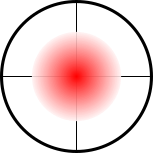
\includegraphics{figs-modalmodel/QPD.pdf}
  \end{center}
  \caption[Diagram of a quadrant photodiode]{Diagram of a quadrant photodiode. The beam is pictured centered on the diode. As the beam is displaced vertically, more photocurrent will be measured by the top two segments than the bottom two. Subtracting the bottom photocurrents from the top ones will provide a measurement of the vertical beam position.}
  \label{fig:QPD}
\end{figure}
Photodetectors are sometimes split into many segments, such as is the case with a so called quadrant photo-detector (QPD). %NL%
In the case of a QPD, the face of the photodetector is split into four equal segments as seen in figure \ref{fig:QPD}. %NL%
Different linear combinations of the photocurrents of these segments can yield different information about the laser beam. %NL%
For example, the vertical displacement of a beam can be determined by subtracting current of the top segments from the bottom segments.

The shape and linear combination of the photodiode segments is treated in the literature\cite{Hefetz:97} as a pupil function $p(x,y)$,  where the photodiode measures a signal
\begin{equation}
S=\frac{\epsilon_0 c}{2}\int \! %NL%
\! %NL%
\dd t \iint\limits_{\text{PD area}}E^\dagger(x,y)p(x,y)E(x,y)\dd x \dd y,
\end{equation}
so for example for a photodetector split along the $y$ axis, $p(x,y)=1$ for $x>0$ and $-1$ for $x<0$.

% show how this is equivalent to an operator

In the language of transverse spatial modes, a split photodetector is measuring the mixing of the \TEM{00} mode with the \TEM{10} mode.\footnote{More precisely, it measures the mixing of all even modes to odd modes and vice versa, with the primary contribution coming from the modes which differ by one mode order.} So in order to model this in the vector space framework, we will need to generalize the demodulation operator to have matrix elements between spatial modes as well as frequency components. %NL%
So we may expand the demodulation operator to include spatial components. %NL%
The spatial matrix elements of the demodulation operator are:
\begin{equation}
\matrixel{mn}{\oper{D}(\Omega)}{kl}=\iint\limits_{\text{PD area}}U_{mn}^\dagger(x,y)p(x,y)U_{kl}(x,y)\dd x \dd y,
\end{equation}
where the ``variable'' %NL%
$\Omega$ is just supposed to contain all the information of the pupil function.\footnote{$\Omega$ does not represent an angular frequency in this case.}

The frequency, spatial, and polarization parts of the demodulation operator and combined simply with a tensor product,
\begin{equation}
\oper{D}(\Omega,\omega_d) = \oper{D}(\Omega)_{\text{modal}}\otimes\oper{D}(\omega_d)_{\text{frequency}}\otimes\oper{I}_{\text{polarization}},
\end{equation}
where $\oper{I}$ is the identity operator.

Once the demodulation operator is constructed, the signal measured by the photodetector is
\begin{equation}
S=\frac{\epsilon_0 c}{2}\matrixel{E}{\oper{D}(\Omega,\omega_d)}{E}.
\end{equation}
In terms of the quantum mechanical analogy, the signal measured on a photodetector is just the expectation value of it's demodulation operator.

\section{Vector space model of the output mode cleaner}
The true utility of this formalism arises when the optical system contains paths that branch and loop onto themselves, as is the case with resonant cavities. %NL%
The fact that the operators can simultaneously handle the transverse modes and frequency components reduces much of the complexity of the problem through abstraction.
\begin{figure}
  \begin{center}
  \leavevmode
  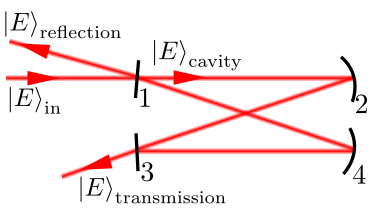
\includegraphics{figs-modalmodel/omcmodal.pdf}
  \end{center}
  \caption[Diagram of vector space model of the OMC]{Diagram of vector space model of the OMC}
  \label{fig:omcmodal}
\end{figure}
%a simple ring cavity
In figure \ref{fig:omcmodal} we see a schematic diagram of a four mirror ring cavity. %NL%
Every interaction of the laser field is handled by an operator. %NL%
This includes transmission through an optic, reflection from an optic, and propagation through free space. %NL%


We may write down an expression for the field inside the cavity as follows
\begin{equation}
\vect{E}_{\text{cavity}} = \oper{T}_1\vect{E}_{\text{input}}+\oper{G}\vect{E}_{\text{cavity'}}.
\end{equation}
Here, $\oper{G}$ is the operator representing one full round trip through the cavity, starting with the propagation from mirror 1 to mirror 2, $\oper{T}_1$ is the operator for transmission through mirror 1, and $\vect{E}_{\text{cavity'}}$ is the cavity field due to the previous round trip of the light. %NL%
When the system has reached a stationary state, $\vect{E}_{\text{input}}=\vect{E}_{\text{cavity'}}$.\footnote{Note that this does not only include fields static in time, but also any peiodically changing fields that are represented in our vector space.} In this case we may solve for the field in the cavity:
\begin{equation}
\vect{E}_{\text{cavity}} = \left(\oper{I}-\oper{G}\right)^{-1}\oper{T}_1\vect{E}_{\text{input}}.
\end{equation}
The round trip operator is 
\begin{equation}
\oper{G} = \oper{P}_{1\rightarrow 2}\oper{M}_2\oper{P}_{2\rightarrow 3}\oper{M}_3\oper{P}_{3\rightarrow 4}\oper{M}_4\oper{P}_{4\rightarrow 1}\oper{M}_1,
\end{equation}
where $\oper{P}_{j\rightarrow j+1}$ is the free space propagation operator from mirror $j$ to $j+1$, and $\oper{M}_k$ is the reflection operator for mirror $k$.

By definition, the mirror operators are all diagonal when the system is aligned. %NL%
Also the propagation operators are diagonal by construction. %NL%
The diagonal matrix elements of $\oper{G}$ vary in their phase from one field component to the next. %NL%
Thus one can see that when these matrix elements have a phase close to an integer multiple of $2\pi$, the cavity field of those components will be enhanced. %NL%
This is of course just the expected resonance behavior. %NL%
As the length of the cavity is changed (which modifies the propagation operators) different field components will come in and out of resonance. %NL%
This includes both frequency components and higher order mode components, indeed different frequency components of different higher order mode components as well!

The following chapter describes an alignment system designed to measure the spatial modes of only a particular frequency component of the laser field. %NL%
The concepts introduced in this chapter are well suited to describe such a system.